\documentclass[12pt]{article}
\usepackage[a4paper, top=2.5cm, bottom=2.5cm, left=2cm, right=2cm]{geometry}
\usepackage{amsmath, amssymb}
\usepackage{graphicx}
\usepackage{cite}
\usepackage{hyperref}
\usepackage{setspace}
\usepackage{lmodern}  % 可选:提高 PDF 输出质量
\usepackage{indentfirst}
\usepackage{cancel}
\usepackage{xcolor}
\usepackage{float}
\numberwithin{equation}{section}
\newcommand{\mdavg}[2]{\langle #1 \rangle\!\langle #2 \rangle}
\newcommand{\avg}[1]{\langle #1 \rangle}
\newcommand{\aket}[1]{|#1\rangle}
\newcommand{\asqu}[1]{{\langle#1\rangle}^2}
\newcommand{\sket}[1]{|#1]}
\newcommand{\cbrak}[2]{\avg{#1}\![#2]}
\newcommand{\acbrak}[2]{[#1]\!\avg{#2}}
\newcommand{\tif}[1]{\textit{\textbf{#1}}}
\onehalfspacing

\begin{document}

\begin{titlepage}
    \centering
    \vspace*{2cm}

    {\LARGE \textbf{On-Shell Methods for Tree-Level Amplitudes in (De)Constructed Gauge Theory}}\\[1.5cm]

    \textbf{Author:} \\
    {\Large Su Yingze} \\[1cm]

    \textbf{Affiliation:} \\
    Department of Physics, Faculty of Science \\
    Nagoya University \\[1cm]

    \textbf{Major:} \\
    Theoretical Physics \\[1cm]

    \textbf{Degree:} \\
    Master of Science \\[1cm]

    \textbf{Submitted on:} \\
    June 2025 \\[2cm]

    \vfill
\end{titlepage}
\newpage
\begin{abstract}
\normalsize
This paper mainly show the computation for scattering amplitudes in a kind of (De)Constructed gauge theory, by using the so called on shell method. As we have known,
under the conventional quantum field theory frame, Feynman proposed a brilliant method -- Feynman diagrams, to help us perturbatively compute scattering amplitude by a
diagrammatic method. However, this method faces many challenges during the improvements of physical theory and complexity of construction for model building, there are many
amplitudes hard to compute by hand or even impossible to compute. Hence, it is quite necessary to introduce a new method.      
\end{abstract}
\newpage
\tableofcontents
\newpage
\section{Introduction}
As we have known,
under the conventional quantum field theory frame, Richard Feynman proposed a brilliant method -- Feynman diagrams, to help us perturbatively compute scattering amplitude by a
diagrammatic method. However, this method faces many challenges during the improvements of physical theory and complexity of construction for model building, there are many
amplitudes hard to compute by hand or even impossible to compute. In gauge theory, there are huge number of gauge redundancies, making the computation quite complicated.
We need to address with this kind of unphysical degree of freedom, otherwise we can not obtain the correct physical quantities. Also, we have to address with kinematic factor and color factor simultaneously in the nonabelian gauge theory.
And it has been known that the amplitudes in $\mathcal{N}=4$ super Yang-Mills theory obtain the symmetry -- dual superconformal symmetry\cite{Drummond:2008vq}, which is not reflected in conventional Feynman diagram method. 

Hence, all of these factors impetus physicists to propose something new, then the BCFW recursion relation is the first product as a new method to compute amplitudes . Historically, the original recursion relation is for gluon scattering amplitudes, coming from Britto, Cachazo and Feng \cite{Britto:2004ap},
and it can be seen as the first breakthrough for modern amplitude method. They explored the analytic properties of amplitudes when extended into complex momentum space. In particular, they considered deforming two external momenta by a complex parameter z, in such a way that the on-shell conditions and momentum conservation are preserved.
Through this deformation, they observed that tree-level amplitudes exhibit simple pole structures in the complex 
z-plane, corresponding to internal propagators going on-shell. This analytic structure allowed them to derive a recursion relation that expresses an 
n-point amplitude in terms of lower-point amplitudes. Edward Witten subsequently noticed that his Twistor String Theory\cite{Witten:2003nn}, which reveals the hidden symmetry and geometry structure of amplitude, implied that the scattering amplitudes has stronger 
analytic property. Their collaboration led to a general formulation of the recursion relations, now known as the BCFW recursion relations\cite{Britto:2005fq}, named after Ruth Britto, Freddy Cachazo, Bo Feng, and Edward Witten.
In particular, Witten helped clarify the large -- z behavior of the amplitudes under complex momentum shifts --- a crucial condition ensuring the validity of the recursion. 

The starting point comes from the precise cancellation in scattering for longitudinal modes of massive spin-2 Kaluza-Klein(KK) states. While individual contributions grow as $\mathcal{O}(s^5)$, $\mathcal{O}(s^4)$, $\mathcal{O}(s^3)$ and $\mathcal{O}(s^2)$, it has been proved that these contributions are cancelled with
each other in a quite intricate way\cite{SekharChivukula:2019yul}, and the final results only grow as $\mathcal{O}(s)$. But it is quite difficult to compute this kind of scattering amplitudes, so if we can obtain some clues for this KK scattering amplitudes from other aspects, it may help us to
understand this cancellation in another way. This paper is motivated by a kind of (De)constructed gauge theory, proposed by Nima, Cohen and Georgi\cite{Arkani-Hamed:2001kyx}. They constructed a renormalizable, asymptotically free, four dimension gauge theories that dynamically generate a fifth dimension. 
In this paper, the authors proposed that the “ Condensed '' theory actually discretized a five dimension gauge theory with gauge group $SU(m)$. After higgsing, the Kaluza-Klein spectrum for $S^1$ compactification appears. It encourages to compute scattering amplitudes in this model. This paper mainly contributes to the 
computation for scattering amplitudes in the simplest 2-site model by utilizing BCFW recursion relation and other related method, such as color-ordered amplitudes, spinor-helicity formalism, etc.

\section{Review of BCFW recursion relation and others}
Traditionally, one relies on Feynman diagrams to calculate scattering amplitudes. Feynman diagrams
provide a clear picture of physics and a systematic procedure of calculations. They are in textbooks
and widely used. But Feynman diagrams are not efficient in complicated calculations for high energy physics. Increasing
the number of particles in a scattering, the number of Feynman diagrams increase exponentially. If gauge
fields are involved, one easily encounters thousands of diagrams. For example, for pure gluon case, the number
of Feynman diagrams for n-gluons at tree-level is given by
\begin{table}[htbp]
    \centering
\begin{tabular}{|c|c|c|c|c|c|c|c|}
    \hline
    n= & 4 & 5 & 6 & 7 & 8 & 9 & 10 \\
    \hline
       & 4 & 25 & 220 & 2485 & 34300 & 559405 & 10525900   \\
    \hline
    \end{tabular}
\end{table}

\noindent
{
(These numbers are counted with the inclusion of 4 point interaction.)}

Not only with huge number
of diagrams, the expression for a single Feynman diagram can also be very complicated. For example, the
three-graviton vertex has almost 100 terms. It is almost impossible to calculate scattering amplitudes of
gravitons directly from Feynman diagrams. For gauge theories, single Feynman diagram usually depends
on the gauge. Many terms cancel with each other at the end of process of calculation. In practice, one does not
even know where to start most times.

BCFW are devised to solve some of these problems. So in the following part, I will give a systematic introduction to BCFW
recursion relation and other necessary tools. This section is mainly based on the excellent review by Elvang and Huang \cite{Elvang:2013cua}.
\subsection{Spinor-Helicity Formalisim for Massless Particles}
\subsubsection{Brief introduction of spinor-helicity formalism}
The spinor-helicity formalism just told us that a light-like Lorentz 4-vector can be decomposed to the product of 
two Weyl spinor. It is quite natural to see it from the representation of Lorentz group. A Lorentz 4-vector lives in $(\frac{1}{2},\frac{1}{2})$ representation,
which can be decomposed to $(\frac{1}{2},0)\bigoplus (0,\frac{1}{2})$. We have known that the $(\frac{1}{2},0)$ and $(0,\frac{1}{2})$ correspond to left handed Weyl spinor and 
right handed Weyl spinor respectively.

Given a null momentum $p_\mu$ in four dimension spacetime, we can define a $2\times2$ matrix by sigma matrix 
\begin{equation*}
    p_{\alpha\dot{\alpha}}=p_\mu\sigma^\mu=\begin{pmatrix}
        p^0-p^3 & -p^1+ip^2\\
        -p^1-ip^2 & p^0+p^3
    \end{pmatrix}
\end{equation*}
note that det$p_{\alpha\dot{\alpha}}=0$ for massless particles, so it is always possible find two Weyl spinor(two components quantity) satsfying the following equation
\begin{equation}
    p_\mu \sigma^\mu=p_{\alpha\dot{\alpha}}=\lambda_\alpha \tilde{\lambda}_{\dot{\alpha}}=\aket{\lambda}[\lambda|
    \label{2.1}
\end{equation}
and similarly we can obtain define
\begin{equation}
    p_\mu \bar{\sigma}^\mu=p^{\dot{\alpha}\alpha}=\tilde{\lambda}^{\dot{\alpha}}\lambda^\alpha=\sket{\lambda} \langle \lambda |,
\end{equation}
For general complex momenta, the $\lambda_\alpha$ and $\tilde{\lambda}_{\dot{\alpha}}$ are independent two dimensional complex vectors. For real momenta, the matrix is Hermitian and 
so we have $\tilde{\lambda}_{\dot{\alpha}}=(\pm)(\lambda_\alpha)^*$.

Thet satisfy the following Weyl equation
\begin{equation}
    p_{\alpha\dot{\alpha}}\sket{p}^{\dot{\alpha}}=0,\quad [p|_{\dot{\alpha}}p^{\dot{\alpha}\alpha}=0,\quad p^{\dot{\alpha}\alpha}\aket{p}_\alpha,\quad \langle p|^\alpha p_{\alpha\dot{\alpha}}=0
\end{equation}
and we can use two-dimension antisymmetric tensor to raise or lower the indices
\begin{equation}
    [p|_{\dot{\alpha}}=\varepsilon _{\dot{\alpha}\dot{\beta}}\sket{p}^{\dot{\beta}},\qquad \langle p|^\alpha=\varepsilon^{\alpha\beta}\aket{p}_{\beta}
\end{equation}
\noindent
Then,

\boxed{\text{The angle and square spinors are the core of \textbf{spinor-helicity formalism}}.}

\vspace{1em}
Here, it is also necessary to introduce the \textbf{angle spinor bracket} $\avg{pq}$ and \textbf{square spinor bracket} $[pq]$, it is the key ingredient for writing amplitudes in terms of spinor-helicity variable.
\begin{equation}
    \avg{pq}=\langle p|^\alpha \aket{q}_\alpha,\qquad [pq]=[p|_{\dot{\alpha}}|q]^{\dot{\alpha}}.
\end{equation}
Since the indices are raised and lowed by antisymmetric tensor, so the brackets are antisymmetric:
\begin{equation}
    \avg{pq}=-\avg{qp},\qquad [pq]=-[qp].
\end{equation}
There are no $\langle pq]$ brackets, because the indices cannot contract with each other to form a Lorentz scalar.

It is very easy to derive the following important relation:
\begin{equation}
    \cbrak{pq}{pq}=2p\cdot q= (p+q)^2
    \label{2.7}
\end{equation}
by using \eqref{2.1} and 
\begin{equation*}
    \mathrm{Tr}(\sigma^\mu \bar{\sigma}^\nu)=2\eta^{\mu\nu}.
\end{equation*}
Here, we list other identities without any provement
\begin{align}
    &[k|\gamma^\mu\aket{p}=\langle p|\gamma^\mu |k],\\
    &{[k|\gamma^\mu\aket{p}}^*=[p|\gamma^\mu\aket{k} \qquad \text{(for real moemnta)}.
\end{align}
and \textbf{Fierz identity}
\begin{equation}
    \langle 1|\gamma^\mu |2]\langle 3|\gamma_\mu |4]=2\cbrak{13}{24}
\end{equation}
will be used in several times.
In amplitude calculations, \textbf{momentum conservation} is imposed on n particles as $\sum_{i=1}^{n}p_i^\mu=0$(here we consider all particles ingoing). Translating by 
spinor-helicity variable, it becomes
\begin{equation}
   \sum_{i=1}^{n}\aket{i}[i|=0,\quad \text{i.e.}\quad \sum_{i=1}^{n}\cbrak{qi}{ik}=0,
\end{equation}
here q and k are arbitrary light-like vectors.

We end this subsection by introducing one more identity: \textbf{Schouten Identity}. It comes from a rather trivial fact: there are no three independent 2-dimensional vectors. So if we have three 2 components angle spinors $\aket{i}$, $\aket{j}$ and $\aket{k}$, we can write one of them as a linear combination of two others
\begin{equation}
    \aket{k}=a\aket{i}+b\aket{j},\qquad \text{for complex a and b}.
    \label{2.8}
\end{equation} 
One can contract a $\aket{i}$ and a $\aket{b}$ with the both sides, then a,b can be solved. \eqref{2.8} can be cast to the form
\begin{equation}
    \aket{i}\avg{jk}+\aket{k}\avg{ij}+\aket{j}\avg{ki}=0,
\end{equation}
This is Schouten identity and often written with a fourth spinor $\langle r|$
\begin{equation}
    \cbrak{ri}{jk}+\mdavg{rk}{ij}+\mdavg{rk}{ki}=0.
\end{equation}
We have a similar Schouten identity holding for square spinors
\begin{equation}
    [ri][jk]+[rk][ij]+[rj][ki]=0.
\end{equation}

There is also a important result can be obtained, the \textbf{3-particle soecial kinematics}. If we have three light-like vectors satisfying momentum conservation
$p_1^\mu+p_2^\mu+p_3^\mu=0$. Then
\begin{equation}
    \mdavg{12}{21}=2p_1\cdot p_2=(p_1+p_2)^2=p_3^2=0,
\end{equation}
so either $\avg{12}$ or $[12]$ equals to 0. If we suppose $\avg{12}\neq0$, then from $\avg{12}[23]=\langle 1|p_2|3]=-\langle 1|p_1+p_3|3]=0$, we can conclude that
$[23]=0$. Similarly, we can also obtain $[31]=0$. Thus, $[12]=[23]=[31]=0$, which means that the three square spinors are proportional with each other
\begin{equation}
    |1] \propto |2] \propto |3]
\end{equation}
or another possibility
\begin{equation}
    \aket{1}\propto\aket{2}\propto\aket{3}.
\end{equation}
As a consequence,
\begin{enumerate}
    \item A non-vanishing on-shell 3-particle amplitude depends only on square brackets or angle brackets.
    \item Since for real momenta, angle brackets are complex conjugated with square brackets, so \textit{on-shell 3 point amplitudes are only meanful for complex momenta}(unless it is a constant, like $\phi^3$ theory).
\end{enumerate}
\subsubsection{Yang-Mills and Color-ordering}
Let us consider the Yang-Mills lagrangian
\begin{equation}
    \mathcal{L}=-\frac{1}{4}F_{\mu\nu}F^{\mu\nu},
\end{equation}
with field strength $F_{\mu\nu}=\partial_\mu A_\nu -  \partial_\nu A_\mu - \frac{ig}{\sqrt{2}}[A_\mu,A_\nu]$, and $A_\mu=A_\mu^a T^a$. Gauge fields belong to adjoint representation, so the index a runs over $1,2 \cdots N^2-1$ in $SU(N)$ case. The generators are normalized like $\textrm{Tr}[T^aT^b]=\delta^{ab}$ and $[T^a,T^b]=i\tilde{f}^{abc}T^c$\footnote{In the usual QFT textbook,
$\textrm{Tr}[T^aT^b]=\frac{1}{2}\delta^{ab}$ and $[T^a,T^b]=if^{abc}T^c$, with $\tilde{f}^{abc}=\sqrt{2}f^{abc}$ are common choice.  }. 

The amplitude-friendly gauge choice is \textit{Gervais-Neveu gauge } with gauge fixing term $\mathcal{L}_{gf}=-\frac{1}{2}\mathrm{Tr}(H_\mu^\mu)=0$, here $H_{\mu\nu}=\partial_\mu A_nu - \frac{ig}{\sqrt{2}}A_\mu A_\nu$.
After gauge fixing, the lagrangian becomes 
\begin{equation}
    \mathcal{L}=\mathrm{Tr} \left(-\frac{1}{2}\partial_\mu A_\nu \partial^\mu A^\nu - i\sqrt{2}g\partial^\mu A^\nu A_\nu A_\mu+\frac{g^2}{4}A^\mu A^\nu A_\mu A_\nu \right)
\end{equation}
The 3- and 4-gluon vertices involve $\tilde{f}^{abc}$ and $\tilde{f}^{abi}\tilde{f}^{icd}$+permutations, respectively, each dressed up with kinematic factors.
The amplitudes constructed from these rules can be organized into
different group theory structures. For example, the
color factors of the s-, t-, and u-channel diagram of the 4-gluon tree amplitude are
\begin{equation}
    c_s=\tilde{f}^{a_1a_2b}\tilde{f}^{ba_3a_4},\quad c_t=\tilde{f}^{a_4a_1b}\tilde{f}^{ba_2a_3},\quad c_u=\tilde{f}^{a_1a_3b}\tilde{f}^{ba_2a_4}
\end{equation}
and the four point interaction just gives a sum of contributions from $c_s$, $c_t$ and $c_u$. And because of the Jacobi identity, we have
\begin{equation}
    c_s=c_t+c_u.
\end{equation}

And the color factor can be written by the trace of product of generators
\begin{equation}
    i\tilde{f}^{abc}=\mathrm{Tr}([T^a,T^b]T^c),
\end{equation}
where $T^a$ are generators of fundamental representation. Moreover, in $SU(N)$, we have a Fierz identity
\begin{equation}
    \sum_{a}T^a_{ij}T^a_{kl}=\delta_{il}\delta_{kj}-\frac{1}{N}\delta_{ij}\delta_{kl}.
\end{equation}
This identity is easier understood as matrix form like 
\begin{equation}
    \mathrm{Tr}\{T^aA\}\mathrm{Tr}\{T^aB\}=\mathrm{Tr}\{AB\}-\frac{1}{N}\{A\}\mathrm{Tr}\{B\},
\end{equation}
and
\begin{equation}
    \mathrm{Tr}\{AT^aBT^a\}=\mathrm{Tr}\{A\}\mathrm{Tr}\{B\}-\frac{1}{N}\mathrm{Tr}\{AB\}.
\end{equation}
Then it can be used to simplify the calculation.

For example, the 4 gluon s-channel gives us
\begin{equation}
    \tilde{f}^{a_1a_2b}\tilde{f}^{ba_3a_4}=\mathrm{Tr}(T^{a_1}T^{a_2}T^{a_3}T^{a_4})-\mathrm{Tr}(T^{a_2}T^{a_1}T^{a_3}T^{a_4})-\mathrm{Tr}(T^{a_1}T^{a_2}T^{a_4}T^{a_3})+\mathrm{Tr}(T^{a_2}T^{a_1}T^{a_4}T^{a_3}).
\end{equation}
Similarly, three other diagrams can also be written in terms of single trace. Therefore, the full 4-point amplitude can be rewritten like
\begin{equation}
    \mathcal{A}_{4,\text{tree}}=g^2(A_4[1234]\mathrm{Tr}(T^{a_1}T^{a_2}T^{a_3}T^{a_4})+\text{perms of } (234) )
\end{equation}
here the subamplitudes $A_4[1234],A_4[1243]$, etc. are called \textbf{color-ordereed ampltitudes}. This concept can be easily generalized to tree-level n-point case
\begin{equation}
    \mathcal{A}_{n,\text{tree}}=g^{n-2}\sum_{\sigma}A_n[1,\sigma(2,3\cdots n)]\mathrm{Tr}(T^{a_1}T^{\sigma(a_2\cdots}T^{a_n)})
    \label{2.29}
\end{equation}
where the sun is taken over the $(n-1)!$ trace basis (considering the cyclic property of trace). Actually, the number of independent basis can be reduced to $(n-3)!$, called Del Duca-Dixon-Maltoni (DDM) color decomposition\cite{DelDuca:1999rs}. But it has no tight relation with this paper, so here we do not offer more detailed explanation for it. 

The color-ordered amplitude $A_n[1,2 ... n]$ is calculated in terms of diagrams with no lines crossing(planar diagrams) and the ordering of the external lines fixed as given 1, 2, 3,..., n. Here, we directly give the final result for 3-point color-ordered amplitudes without any intermediate calculating process. And in this full paper, we mainly consider the helicity amplitudes which will be explained later, so we need to clarify the helicity configuration.

For 3-point, there are only two non-vanishing configurations
\begin{equation}
    A_3[1^-,2^-,3^+]=\frac{\avg{12}^3}{\mdavg{23}{31}}
\end{equation}
and 
\begin{equation}
    A_3[1^+,2^+,3^-]=\frac{[12]^3}{[23][31]}.
\end{equation}

It has been known that there is a compact formula for n-point gluon color-ordered amplitudes --- \textbf{\textit{Parke - Talyor Formula}}
\begin{equation}
    A_n[1^+\cdots i^-\cdots j^- \cdots n^+]=\frac{\avg{ij}^4}{\mdavg{12}{23}\cdots\avg{n1}}.
\end{equation}
We will prove this formula in the next subsection.

The color-ordered amplitudes have a number of properties
\begin{enumerate}
    \item \textit{Cyclic}: It follows from the cyclic property for trace that $A_n[12\cdots n]=A_n[2n\cdots 1]$
    \item \textit{Reflection}: $A_n[12\cdots n]=(-1)^nA_[n\cdots 21]$
    \item The $U(1)$ \textit{decoupling identity}: 
    \begin{equation}
        A_n[123\cdots n]+A_n[213\cdots n]+A_n[231\cdots n]+\cdots + A_n[23\cdots 1n]=0
    \end{equation}
\end{enumerate}

The trace basis \eqref{2.29} is overcomplete implies that there are further linear relations among these subamplitudes, which are called 
\textit{\textbf{Kleiss - Kuiff(KK) relations}} 
\begin{equation}
    A_n[1,\{\alpha\},n,\{\beta\}]=(-1)^{|\beta|}\sum_{\sigma\in \text{OP}(\{\alpha\},\{\beta^T\}) }A_n[1,\sigma,n]
\end{equation}
where $\beta^T$ denotes the reverse ordering of the labels $\{\beta\}$  and the sum is over ordered
permutations “OP”, means permutations of the labels in the joined set $\{\alpha\}\cup \{\beta^T\}$ in which 
the ordering within $\{\alpha\}$ and $\{\beta\}^T$ is preserved. 

Consider a 5-point case as an example. Taking the LHS to be $A_5[1,\{2\},5,\{3,4\}]$, we have $\{\alpha\}\cup \{\beta^T\}=\{2\}\cup \{4,3\}$, so the 
ordered permutations $\sigma$ refers to $\{243\},\{423\},\{432\}$. Thus the KK relation reads
\begin{equation}
    A_5[12534]=A_5[12435]+A_5[14235]+A_5[114325].
\end{equation}

The KK relations combine with cyclic, reflection, and $U(1)$ decoupling identities reduce the number of independent
basis to $(n-2)!$. However, there are further linear relations called $\textit{\textbf{BCJ relations}}$ -- named after Bern, Carrasco and Johansson, which further
reduce the number to $(n-3)!$. 

Although I will not show the derivation of BCJ relations, I would like to give some examples
\begin{gather}
    s_{14}A_4[1234]-s_{13}A_4[1243]=0,\\
    s_{12}A_5[21345]s_{23}A_5[13245]-(s_{23}+s_{24})A_5[13425]=0.
\end{gather}
\subsection{Little group scalling}
The rich structure of scattering amplitudes can be originated from a fundamental question — “What is a particle?” — which relates directly to Wigner’s Little group notation,
characterizing how particles transform under Lorentz symmetry. Following this thought, we think particle as a unitary representation of 
Poincar$\acute{e}$ group, which is the symmetry group of our spacetime. We use two labels to denote a one-particle state, one is the momentum $p^\mu$, another is $\sigma$ representing
other labels the particle ca carry. 

We start from a one-particle state $\aket{k;\sigma}$ with reference momentum $k$. Another momentum $p$ is related by the lorentz transformation $L(p;k)$, $p=L(p;k)k$. Obviously, this Lorentz transformation is
not unique because there exist Lorentz transformations keeping p invariant, called ``Little group transformation''.  We assume that there exist a 
unitary representation for the Lorentz group, the operator in Hillbert space are denoted like $U(\Lambda)$. 

Then we simply \textit{define} the one-particle state with momentum p as 
\begin{equation}
    \aket{p;\sigma}=U(L(p;k))\aket{k;\sigma}.
\end{equation}
Having made this definition, we can compute how the state transformed under a general Lorentz transformation
\begin{equation}
    U(\Lambda)|p,\sigma\rangle = U(\Lambda) U(L(p;k))|k,\sigma \rangle = U(L(\Lambda p;k)) U(L^{-1}(\Lambda p;k) \Lambda L(p;k)) |k,\sigma \rangle\,.
\end{equation}
here we use the fact $U(\Lambda_1\Lambda_2)=U(\Lambda_1)U(\Lambda_2)$.
Notice that $W(\Lambda,p,k)$ is not a general transformation but keep the momentum k invariant $Wk=k$. This subgroup of Lorentz group is called little group.
Thus we must have 
\begin{equation}
    U(W(\Lambda,p,k))\aket{k;\sigma}=D_{\sigma\sigma^{'}}(W(\Lambda,p,k))\aket{k,\sigma^{'}},
\end{equation} 
where $D_{\sigma\sigma^{'}}$ is the representation for little group. Then, p should transformed like
\begin{equation}
     U(\Lambda)|p,\sigma\rangle=D_{\sigma\sigma^{'}}(W(\Lambda,p,k))\aket{\Lambda p,\sigma^{'}}
\end{equation}

The scattering amplitudes for n particle should keep invariant under Poincar$\acute{e}$ transformation -- translation invariance and Lorentz invariance
\begin{gather}
    \mathcal{M}(p_a,\sigma_a)=\delta^D(p_1^\mu+\cdots +p_n^\mu)\mathcal{M}(p_a,\sigma_a)\\
    \mathcal{M}^\Lambda(p_a,\sigma_a)=\prod_{a}(D_{\sigma\sigma^{'}})\mathcal{M}((\Lambda p)_a,\sigma_a^{'})
    \label{2.43}
\end{gather}

In D spacetime dimensions, the little group for massive particles is $SO(D-1)$. For massless
particles the little group is the the group of Euclidean symmetries in (D - 2) dimensions, which
is $SO(D-2)$.In this article, we mainly discuss massless particles scattering in 4 dimension spacetime, so the little group is $SO(2)\backsimeq U(1)$.

Then from the definition of spinor-helicity variable\eqref{2.1}, we can notice that there is an ambiguity here.
The momentum is invariant under the following redefinition
    \begin{equation}
        \lambda \rightarrow t^{-1}\lambda, \qquad \tilde{\lambda}\rightarrow t\tilde{\lambda}, \qquad t\in\mathbb{C} 
    \end{equation}
    same for
    \begin{equation}
        \aket{\lambda}\rightarrow t^{-1}\aket{\lambda}, \qquad \sket{\lambda}\rightarrow t\sket{\lambda}
    \end{equation}.
This scale perfectly matches the $U(1)$ little group transformation, so we can identify this rescale as the little group transformation.
The scattering amplitudes should transform \textcolor{red}{covariantly} under little group scaling like \eqref{2.43}, so
\begin{equation}
    \color{red} \mathcal{A}_n(\{\aket{1},\sket{1},h_1\},\ldots\{t_i^{-1}\aket{i},t_i\sket{i},h_i\},\ldots )=t_i^{2h_i}\mathcal{A}_n
    \label{2.46}
\end{equation}
where $h_i$ refers to the helicity of particles.
As an example, consider the QED amplitude, $A_3(f^-\bar{f}^+\gamma^-)=e\frac{\avg{13}^2}{\avg{12}}$. For the negative helicity photon (particle 3), we obtain $t_3^{-2}=t_3^{2(-1)}$.
We will see that little group scaling plays a significant role in 3-particle amplitudes.

\noindent
\textbf{3-particle amplitudes}

\noindent
By 3-particle special kinematics, we have known that on-shell 3-point amplitudes depends on either square brackets or
angle brackets. We suppose that it only depends on angle brackets. We can write down the general ansatz
\begin{equation}
     A_3(1^{h_1},2^{h_2},3^{h_3})=c\avg{12}^{x_{12}}\avg{13}^{x_{13}}\avg{23}^{x_{23}},
\end{equation}
where c is just a constant. Little group scaling \eqref{2.46} tell us that
\begin{equation}
    t_1^{2h_1} A_3(1^{h_1},2^{h_2},3^{h_3})=ct_1^{-x_{12}}t_1^{-x_{13}}\avg{12}^{x_{12}}\avg{13}^{x_{13}}\avg{23}^{x_{23}}.
\end{equation}
We can obtain
    \begin{equation}
        2h_1=-x_{12}-x_{13}
    \end{equation}
    Similarly, we can also obtain
    \begin{equation}
        2h_2=-x_{12}-x_{23},\qquad 2h_3=-x_{13}-x_{23}.
    \end{equation}
    Then all index can be solved from this system of equations, so that
 \begin{align}
    A_3^{h_1h_2h_3} &= c\langle12\rangle^{h_3-h_1-h_2} \langle31\rangle^{h_2-h_1-h_3} \langle23\rangle^{h_1-h_2-h_3}
    && \quad h_1 + h_2 + h_3 < 0 \label{2.51}\\[0.5em] 
    A_3^{h_1h_2h_3} &= c' [12]^{h_1+h_2-h_3}[23]^{h_2+h_3-h_1}[31]^{h_3+h_1-h_2}
    && \quad h_1 + h_2 + h_3 > 0 \label{2.52}
\end{align}
This means that \textit{\textbf{all massless 3-point amplitudes are completely fixed by little group scaling!}}

We have shown the 3-point QED amplitudes. So now we can consider something different -- 3-point gluon amplitudes with 2 same helicities and 1 different helicity.
Then we can determine the amplitudes from \eqref{2.51} \eqref{2.52}
\begin{equation}
    A_3(g_1^-,g_2^-,g_3^+)=g\frac{\avg{12}^3}{\avg{23}\!\avg{31}}, \quad A_3(g_1^+,g_2^+,g_3^-)=g\frac{[12]^3}{[23][31]} \label{2.53}
\end{equation}

Here it need some efforts to explain about the condition after equation \eqref{2.51} and \eqref{2.52}.If we assume the amplitude
$A_3(g_1^-,g_2^-,g_3^+)$ depending on square brackets, so can obtain a different expression
\begin{equation}
    A_3(g_1^-,g_2^-,g_3^+)=g^{'}\frac{[31][23]}{[12]^3},
    \label{2.54}
\end{equation}
to distinguish these two possibilities, we need to use \textbf{dimension analysis}. From \eqref{2.7}, we can know that both square brackets and angle brackets have mass-dimension 1. 
Thus the kinematic factor of amplitude \eqref{2.53} has mass-dimension 1, compatible with the interaction term $AA\partial A$ in $\mathrm{Tr}F_{\mu\nu}F^{\mu\nu}$. But the mass-dimension 
of kinematic factor in \eqref{2.54} is (-1), so it should come from the interaction term like $g^{'}AA\frac{1}{\square }A$. Here, we only consider the local field theory, so this kind of interaction
should be discarded.

The combination of \tif{little group scaling} and \tif{locality} uniquely fixes the massless 3-point amplitudes. In general, 
\begin{equation}
    \text{An n-point amplitude in D=4 spacetime have mass-dimension 4 - n.}
\end{equation}
Although we discard the amplitude \eqref{2.54}, the coupling s¥constant $g^{'}$ have mass-dimension 2, so \eqref{2.54} has the correct mass-dimension as \eqref{2.53}.

How about the gluon amplitude with all minus helicities? The formula \eqref{2.51} immediately tells that it should equal to
\begin{equation}
    A_3(g_1^-,g_2^-,g_3^-)=g^{''}\mdavg{12}{23}\!\avg{31}.
\end{equation}
The kinematic part has mass-dimension 3 and reveals that: 
\begin{enumerate}
    \item The coupling constant $g^{''}$ must have mass-dimension -2.
    \item This must come from an interaction term with 3 derivatives like $(\partial A)^3$.
\end{enumerate}
Furthermore, kinematic part has the antisymmetry under the exchange of gluon momenta, so the coupling constant should 
also have this antisymmetry in order to satisfy the Bose statics as is of course the pure Yang-Mills case. 
The natural candidate of this amplitude is a dimension 6 operator $\mathrm{Tr}F^\mu_\nu F^\nu_\lambda F^\lambda _\mu$. 

\subsection{MHV Classification}
It has been well known that the all-plus tree-level gluon amplitudes vanish
\begin{equation}
    \text{tree-level gluon amplitues}: \quad A_n[1^+,2^+,\cdots,n^+]=0 \quad\text{and}\quad A_n[1^+,2^+,\cdots,n^-]=0
\end{equation}
This conclusion holds for the case with all helicities flipped:
\begin{equation}
    \text{tree-level gluon amplitues}: \quad A_n[1^-,2^-,\cdots,n^-]=0 \quad\text{and}\quad A_n[1^-,2^-,\cdots,n^+]=0
\end{equation}
In supersymmetric Yang-Mills theories, these results hold for all loop order, so actually it is a special case for SYM.

If we flip one more helicit, the situation becomes quite different. Amplitudes $A_n[1^-,2^-,3^+,\cdots,n^+]$ does not equal to 0 and is quite important called \textbf{MHV amplitudes}.
The gluon amplitudes with two negative helicities and n - 2 positive helicities are called
\tif{maximally helicity violating} – or simply \tif{MHV} for short. The concept ``maximally helicity violating'' comes from thinking a $2\rightarrow n-2$ scattering process. 
Because of crossing symmetry, the outgoing particle with positive(negtive) helicity is equivalent with an ingoing particle with negative(positive) helicty. So if we consider the process $A_n[1^+,2^+,\cdots,n^+]$ with 
all particle ingoing. It crosses over to $1^+2^-+\rightarrow 3^-\cdots n^-$ with two ingoing particles and n-2 outgoing particles, that's the reason we call it ``helicity violating''. We have known that the process in which the most we can violate helicity
is $1^+2^+\rightarrow 3^+4^+5^-\cdots n^-$, which is equivalent to amplitudes $A_n[1^+2^+3^-4^-5^+\cdots n^+]$, therefore it is the \textit{maximally helicity violating} process.

As we have shown in the last subsection, the MHV gluon tree amplitudes are given by Parke - Talyor formula
\begin{equation}
    A_n[1^+\cdots i^-\cdots j^- \cdots n^+]=\frac{\avg{ij}^4}{\mdavg{12}{23}\cdots\avg{n1}}
\end{equation}
The MHV amplitudes are the important blocks for scattering amplitudes in (super)Yang-Mills theory. They are simplest amplitudes, and the next-to simplest
are called \textbf{Next-to-MHV} amplitudes, or just \textbf{NMHV}. This refers to scattering process for which two 2 positive gluons scatter into 3 positive gluons and n-5 negative gluons. 
Similarly, we can define \textbf{$N^k$MHV} amplitudes. For anti-MHV amplitudes with all helicities flipping, we have a formula
\begin{equation}
    A_n[1^-\cdots i^+\cdots j^+ \cdots n^-]=\frac{[ij]^4}{[12][23]\cdots[n1]}.
\end{equation}
\subsection{BCFW recursion relation}
The BCFW recursion relation was introduced in 2005 by Britto, Cachazo, and Feng, and later extended with Witten. It provided a novel way to compute tree-level scattering amplitudes by 
analytically continuing external momenta into the complex plane and expressing higher-point amplitudes recursively in terms of lower-point ones. This on-shell approach uncovered surprising 
simplicity in gauge theory amplitudes and offered an alternative to the traditional Feynman diagram expansion. The method was inspired in part by Witten's twistor string theory and the MHV 
diagram program. In parallel, off-shell recursion relations were also being explored, especially in background field methods and Berends-Giele recursion, which organize amplitudes based on 
off-shell currents. While off-shell methods remain useful in certain computational frameworks, the BCFW recursion highlighted the power of staying strictly on-shell, leading to a deeper understanding 
of symmetry, analyticity, and the geometry of scattering processes. It has since become a cornerstone of modern amplitude research.

Beyond BCFW, other on-shell recursion relations have also emerged—for instance, the KLT relations linking gauge and gravity amplitudes, and the double copy structure as well as recursion 
for theories with special helicity configurations or massive particles. Together, these developments form the foundation of modern amplitude methods, emphasizing physical principles like unitarity, analyticity, 
and factorization over traditional Lagrangian-based techniques.

\subsubsection{Complex shift and Relation from Simple Cauchy's Theorem}
An on-shell amplitude(each external leg satisfies on-shell condition) is labeled by their external momentum $p_\mu$ and hilicity $h_i$.
Here we only consider the massless particles $p_i^2=0$, for $i=1,2,\cdots,n$. And momentum conservation $\sum_{i=1}^{n}p_i^\mu=0$ should hold.

First, let us consider the most general case. We need to introduce n complex-valued vectors $r_i^\mu$ subject to 
\begin{itemize}
    \item $\sum_{i=1}^{n}r_i^\mu=0$,
    \item $r_i\cdot r_j=0$ for all $i,j=1,2,\cdots ,n$. In particular, $r_i^2=0$,
    \item $p_i\cdot r_i=0$ for each i(no sum).
\end{itemize}
These vectors $r_i$ are used to define n shifted momentum
\begin{equation}
    \hat{p}_i^\mu\equiv p_i^\mu+zr_i^\mu\quad \text{with}\quad z\in \mathcal{C}
\end{equation}
Note that, by imposing these constraints,
\begin{itemize}
    \item Momentum conservation holds for the shifted momentum: $\sum_{i=1}^{n}\hat{p}_i^\mu=0$,
    \item We have $\hat{p}_i^2=0$, so each shifted momentum still keep on-shell
    \item For a non-trival \footnote{non-trival here means at least two and no more than n-2 such that $P_I^2\neq 0$} subset of momentum $\{p_i\}_{i\in I}$,
    define $P_i^\mu=\sum_{i\in I}p_i^\mu$. Then $\hat{P}_I^2$ is \textbf{linear} in z:
    \begin{equation}
        \hat{P}_I^2=P_I^2 -2zP_I\cdot k=-\frac{P_I^2}{z_I}(z-z_I)
    \end{equation}
    beacuse the $z^2$ term vanishes. We can write 
    \begin{equation}
        \hat{P}_I^2=-\frac{P_I^2}{z_I}(z-z_I)\quad \text\quad {with} z_I=\frac{P_I^2}{2P_I\cdot k}
        \label{2.63}
    \end{equation}
\end{itemize}
If we consider the original amplitude $A_n$ in terms of the shifted momentum $\hat{p}_i^\mu$ instead of original momentum. Then the amplitude can be seen as 
a holomorphic function of z. Actually, if we set $z=0$, we can obtain the origin ampltide $A_n=\hat{A}_n(z=0)$.

In this paper, we only focus on the tree-level scatterung amplitudes, in which case the analytic structure becomes quite simple. The tree amplitudes does not have any branch cuts -- there are no 
logs, no square roots, etc.. The tree-level amplitude is a rational function of Lorentz invariant kinematic quantities, like the contraction between momentum or momentum and polarization vector. 
Therefore, the analytic structure can be completely captured by its single poles in the complex z plane. To see that all of the poles are single, we just need to notice 
that we can only ontain poles from propagators. But we have seen that all of the poles can be dertermined by  \eqref{2.63}. 
So $1/\hat{P}_I^2$ gives a single pole at $z_I$, and for generic momentum, $P_I^2\neq 0$(propagator is off-shell) so $z_I\neq 0$. Hence, 
$\hat{A}_n(z)$ only has single poles away from the orignal poine $z=0$.\footnote{Here we need to impose locality to ensure all of the poles can be determined by the propagators.} 

Then let us turn to define a new holomorphic function $\frac{\hat{A}_n(z)}{z}$ in the complex plane. We can pick a contour surrounding the original point 
$z=0$ which is a single pole of this function. The residue of this single pole can be easily computed
\begin{equation}
    \mathrm{Res}|_{z=0}\frac{\hat{A}_n(z)}{z}=\hat{A}_n(z=0)=A_n,
\end{equation}
It is just the unshifted amplitude what we want to compute at the begining. 

Also, we can choose another countour surrounding all single poles, then Cauchy's theorem just tell us 
\begin{equation}
    A_n = - \sum_{z_I} \mathrm{Res}_{z=z_I} \frac{\hat{A}_n(z)}{z}  + B_n\,,
\end{equation}
where the $B_n$ is the residue at $z=\infty$ infinity, called bounday term. By taking $z\rightarrow 1/\omega$, it is easy to notice that
$B_n$ is the $O(z^0)$ term in the $z\rightarrow \infty$ expansion of $A_n$.

\begin{figure}[htbp]
    \centering
    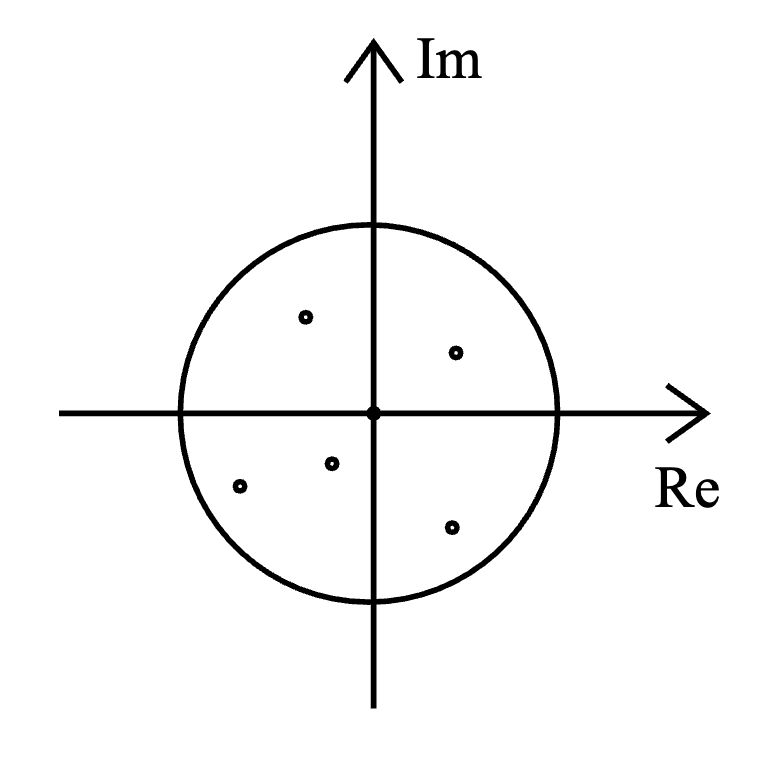
\includegraphics[width=0.5\textwidth]{Cau.png} % 调整为所需大小
    \caption{Cauchy Theorem}
\end{figure}

Now, at the position of $z_I$ pole, the propagator $1/\hat{P}_I^2$ gose on-shell. The unitarity has a tight relation with I poles in the S-matrix with on-shell intermediate
states.
\begin{equation}
    G_n(p_1, \ldots, p_n) = (2\pi)^4 \, \delta^4\left(\sum p\right) 
\frac{i}{p_\Psi^2 - m_\Psi^2 + i\varepsilon} 
\mathcal{M}_\Psi^{1,r} \, \mathcal{M}_\Psi^{r+1,n\dagger} + \text{extra}
\end{equation}
where “extra” refers to anything else that contributes. This equation says that Green’s
functions always have poles when on-shell intermediate particles can be produced. 

Then, in the on-shell limit, the shifted amplitude \textit{factorizes} into two on-shell parts
\begin{equation}
     \hat{A}_n(z)\quad \xrightarrow{z\,\text{near}\,z_I} \quad \hat{A}_L(z_I)\frac{1}{\hat{P}_I^2}\hat{A}_R(z_I)= - \frac{z_I}{z-z_I}\hat{A}_L(z_I)\frac{1}{P_I^2}\hat{A}_R(z_I)
\end{equation}

This makes it easy to compute the residue at $z=z_I$
\begin{equation}
    -\mathrm{Res}|_{z=z_I}\frac{\hat{A}_n(z)}{z}=-(z-z_I)\frac{z_I}{z(z-z_I)}|_{z=z_I}\hat{A}_L(z_I)\frac{1}{P_I^2}\hat{A}_R(z_I)=\hat{A}_L(z_I)\frac{1}{P_I^2}\hat{A}_R(z_I)
\end{equation}

\begin{figure}[H]
    \centering
    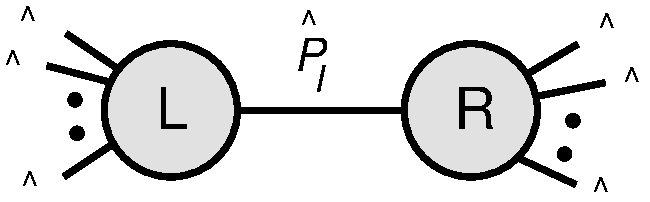
\includegraphics[width=0.5\textwidth]{recrel1.pdf} % 调整为所需大小
    \caption{factorization}
\end{figure}

Note that, as opposed to Feynman diagrams for which the intermediate propagator does not equal to 0, here the intertal line $\hat{P}_I^2$ of Figure 2 does equal to 0.
And the blobs which refer to subamplitudes are \tif{on-shell amplitudes}. In the diagrammatic representation Figure 2, the internal line is assigned the usual scalar propagator 
$1/P_I^2$, evaluated using unshifted momenta. Since each subamplitude involves fewer than 
n external particles, all the residues at finite z can be expressed entirely in terms of lower-point on-shell amplitudes. 
This fundamental idea underlies the construction of the recursion relations.

The contribution $B_n$ does affect a lot, and it has no similar general expression in trems of lower-point amplitudes. Although in some cases, the boundary term
$B_n$ can be computed, but there is not a general method to compute it. Thus, in most applications, we always assumes, or better, prove that $B_n=0$. This is often modified
by demonstrating stronger statement that 
\begin{equation}
    \hat{A}_n(z) \to 0 ~~~~ \text{for} ~~~~ z \to \infty. 
    \label{2.69}
\end{equation}
If \eqref{2.69} holds, we state the shift is \tif{valid}.

For a valid shift, the n-point amplitudes can be recursively computed interms of lower-point amplitude
\begin{equation}
     A_n ~= \sum_{\text{diagrams}~I} \hat{A}_\text{L}(z_I) 
    \,\frac{1}{P_I^2}\,
    \hat{A}_\text{R}(z_I)
       ~~=
   \sum_{\text{diagrams}~I}
   \raisebox{-5.5mm}{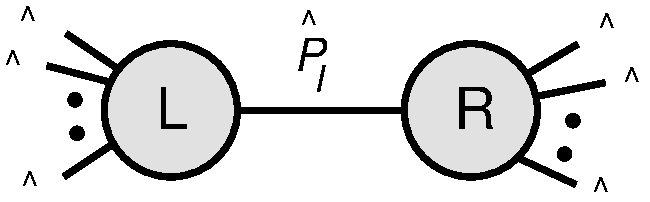
\includegraphics[height=1.4cm]{recrel1}}
   \,.
\end{equation}
where I means all possible factorization channels. We did not use any $D=4$ spacetime property, so this recursion relation can be 
utilized to general D dimension spacetime.

\subsubsection{BCFW recursion relation}
In the last section, we introduce the recursion relation with all momentum shifted. But actually, some of the shift vectors $r_i^\mu$ can be choose to 0.
The BCFW shift is a kind of special shift for which only two momentum are shifted, called i and j. In D=4 spacetime diension, the shift is implemented 
\begin{equation}
    \hat{p}_i(z)=p_i-zq,\qquad \hat{p}_j(z)=p_j+zq
    \label{2.71}
\end{equation}
so momentum conservation is kept and the hold for on-shell condition require ot impose
\begin{equation}
    q^2=q\cdot p_i=q\cdot p_j=0 \, .
\end{equation}
This shift can be implemented in terms of spinor-helicity variable as
\begin{equation}
    |\hat{i}] = |i] - z\,|j]\,,   
  ~~~~~~
  |\hat{j}] = |j]\,,   
  ~~~~~~
  |\hat{i}\rangle = |i\rangle\,,
  ~~~~~~
  |\hat{j}\rangle = |j\rangle + z |i\rangle \,.
\end{equation}
No other spinors are shifted, this kind of shift are called $[i,j\rangle$ shift(it is worth to mention that $[i,j\rangle$ shift 
is completely different with $[j,i\rangle$ shift). In the literature, the BCFW
deformation is usually written in the above spinor form. However, the momentum form \eqref{2.71} provides
another perspective.

The BCFW recursion relation takes the form
\begin{equation}
     A_n ~= \sum_{\text{diagrams}~I} \hat{A}_\text{L}(z_I) 
    \,\frac{1}{P_I^2}\,
    \hat{A}_\text{R}(z_I)
       ~~=
   \sum_{\text{diagrams}~I}
   \raisebox{-5.8mm}{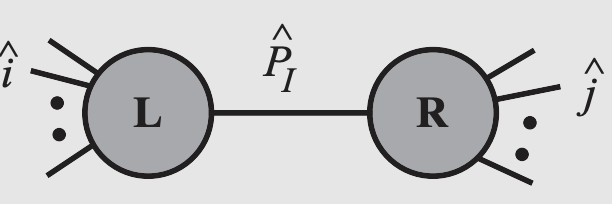
\includegraphics[height=1.4cm]{recrel.2.png}}
   \,.
\end{equation}

Beforing going into the apllication of BCFW, let us first consider the large-z behavior. 
In pure Yang-Mills case, it has been proved that the color-ordered gluon tree-level amplitudes behave like the following manner\cite{Arkani-Hamed:2001kyx}
$$ 
\begin{array}{cccccc}
   [i,j\rangle & [-,-\rangle & [-,+\rangle & [+,+\rangle & [+,-\rangle &
   \\[2mm]
   \hat{A}_n(z) \sim 
   &  \frac{1}{z} &  \frac{1}{z} &  \frac{1}{z} & z^3
   \end{array}
$$
If i,j are not adjacent, one obtains an extra $1/z$ in each case. Thus any one of shifts $,[-,-\rangle,[-,+\rangle,[+,+\rangle$ are valid
but $[+,-\rangle$ is not valid. This is a quite non-trival result.





\newpage
\bibliographystyle{unsrt}
\bibliography{reference.bib}


\end{document}
